\chapter{Results}

This chapter presents the findings of the experiments conducted in this master's thesis. The chapter is divided into two sections.
The first section presents the results of\methodOne{1}, and the second section presents the results of \methodTwo{2}, where both methods will be evaluated in the context of both Gaussian VAEs and VQ-VAEs. In the final section, I will present the cross-validation results of both methods.

\section{Results of \methodOne{1}}

In this section, I will present the results of \methodOne{1} on both Gaussian VAEs and VQ-VAEs.

\subsection{Results on Gaussian VAEs}

The experiments showed similar results for both exact sampling and uniform sampling. The results showed that \methodOne{1} can be used not only to obtain a conditioned decoder but also to improve the quality of non-conditioned decoder reconstruction when compared to non-conditioned Gaussian VAEs. However, KL divergence loss of the latent space increased when \methodOne{1} was applied. This can be explained by the fact that there is a trade-off between the quality of the reconstruction and the KL divergence of the latent space. An example of this can be seen in the figure \ref{fig:results_method1_gaussian_vae}. 

The reconstruction loss of the conditioned decoder was improved when compared to the non-conditioned decoder \ref{fig:res_val}.

To validate and verify that the results are not influenced due to the architecture of the neural network, I applied a range of loss-balancing techniques such as coefficient balancing and the SoftAdapt algorithm. After applying these techniques it could still be observed that the quality of the reconstruction was improved at the expense of a slightly higher KL divergence loss of the latent space. When comparing the results of the Exact Same Sampling and Uniform Sampling it showed little difference to each other.

When trying to use deeper neural networks on the Gaussian VAEs, I observed that the posterior collapse was more likely to happen, which is a common problem in Gaussian VAEs~\cite{wang2023posterior}.
% Think about Coefficients the number of pixels to be sampled. How it changes the results.

\begin{figure}[H]
    \centering
    \centering
\scriptsize
\begin{tabular}{||c|c|c|c||}
\hline
 Method & Parameters & Reconstruction loss & KL loss \\
\hline
\textit{Baseline} & - & 0.0042 +- 1.2e-03 & 0.0018 +- 6.3e-04 \\
\hline
Multi Decoder & Exact sampling & 0.0036 +- 8.3e-04  $\downarrow$ & 0.0027 +- 8.7e-04  $\uparrow$ \\
\hline
Multi Decoder & Exact sampling, SoftAdapt & 0.0034 +- 1.9e-04  $\downarrow$ & 0.0029 +- 2.8e-03  $\uparrow$ \\
\hline
Multi Decoder & Uniform sampling & 0.0035 +- 6.5e-04  $\downarrow$ & 0.0026 +- 1.7e-03  $\uparrow$ \\
\hline
Multi Decoder & Uniform sampling, SoftAdapt & 0.0034 +- 7.3e-03  $\downarrow$ & 0.0029 +- 2.0e-02  $\uparrow$ \\
\hline
\end{tabular}

    \caption[Trained neural network with \methodOne{1} applied to a Gaussian VAE.]
    { 
        Trained neural network with \methodOne{1} with Exact Same Sampling applied to a Gaussian VAE on CelebA dataset and latent space 16. 
        On the left side as input is the original image, on the right side there are two outputs of the decoders. 
        The image from the conditioned decoder is reconstructed with higher quality compared to the non-conditioned decoder because the conditioned decoder $Decoder_2$ uses conditioning information $m$ to improve the quality of the reconstruction.
    }
    \label{fig:res_val}
\end{figure}


\begin{figure}[H]
    \centering
    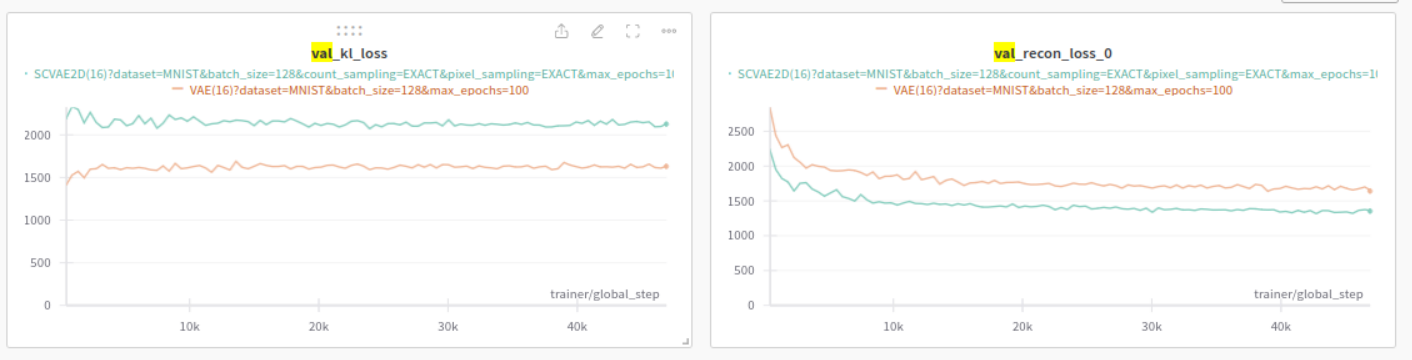
\includegraphics[width=0.8\textwidth]{figures/results/KL_and_RECON.png}
    \caption[Validation loss during training of a Gaussian VAE.]
    {
        Validation losses during training with and without \methodOne{1} applied on Gaussian VAE.
        Left: KL divergence loss of the latent space comparison. Right: Reconstruction loss comparison of the $Decoder_1$ - non-conditioned decoder.
    }
    \label{fig:results_method1_gaussian_vae}
\end{figure}

\subsection{Results on VQ-VAEs}

When applying \methodOne{1} to VQ-VAEs, the results showed that both the quality of the reconstruction and the VQ objective loss improved, which could be observed for both Exact Same Sampling and Uniform Sampling, as shown in figure \ref{fig:results_method1_vq_vae}. This could be explained by the fact that the VQ-VAEs are more robust and stable compared to Gaussian VAEs.

The conditioned decoder was able to reconstruct the image with a higher quality compared to the non-conditioned decoder, however, the difference observed was not as significant as in the Gaussian VAEs. The reasoning behind this lies in the fact that the VQ-VAEs already have a high-quality reconstruction, which makes it harder to improve the quality of the reconstruction.

Same as previously mentioned the method was applied with the SoftAdapt loss balancing technique and without it. The results showed little to no difference between the two. However, the training stability was improved when using SoftAdapt with fewer fluctuations in the loss. When looking at the differences between the Exact Same Sampling and Uniform sampling it showed very little difference between the two, however, the Uniform sampling showed slightly better results.

\begin{figure}[H]
    \centering
    \centering
\scriptsize
\begin{tabular}{||c|c|c|c||}
\hline
 Method & Parameters & Reconstruction loss & VQ loss \\
\hline
\textit{Baseline} & - & 0.0022 +- 7.4e-08 & 0.0029 +- 4.1e-07 \\
\hline
Multi Decoder & Exact sampling & 0.0017 +- 6.9e-09  $\downarrow$ & 0.0039 +- 9.8e-07  $\uparrow$ \\
\hline
Multi Decoder & Exact sampling, SoftAdapt & \textbf{0.0013 +- 2.4e-09}  $\downarrow$ & \textbf{0.0016 +- 6.8e-08}  $\downarrow$ \\
\hline
Multi Decoder & Uniform sampling & 0.0018 +- 1.3e-07  $\downarrow$ & 0.0036 +- 3.5e-07  $\uparrow$ \\
\hline
Multi Decoder & Uniform sampling, SoftAdapt & \textbf{0.0017 +- 6.6e-08}  $\downarrow$ & \textbf{0.0021 +- 3.1e-07}  $\downarrow$ \\
\hline
\end{tabular}

    \caption[Trained neural network with \methodOne{1} applied to a VQ-VAE.]
    {
        Trained neural network with \methodOne{1} and with the Exact Same Sampling applied to a VQ-VAE on the CelebA dataset. The neural network has a latent space of 32 and a table of 128 embeddings, with both the encoder having 4 residual layers and the decoder having 4 residual layers.
        On the left side as input is the original image, on the right side there are two outputs of the decoders. 
        The image from the conditioned decoder is reconstructed with higher quality compared to the non-conditioned decoder because the conditioned decoder $Decoder_2$ uses conditioning information $m$.
    }
    \label{fig:res_val_vqvae}
\end{figure}

\begin{figure}[H]
    \centering
    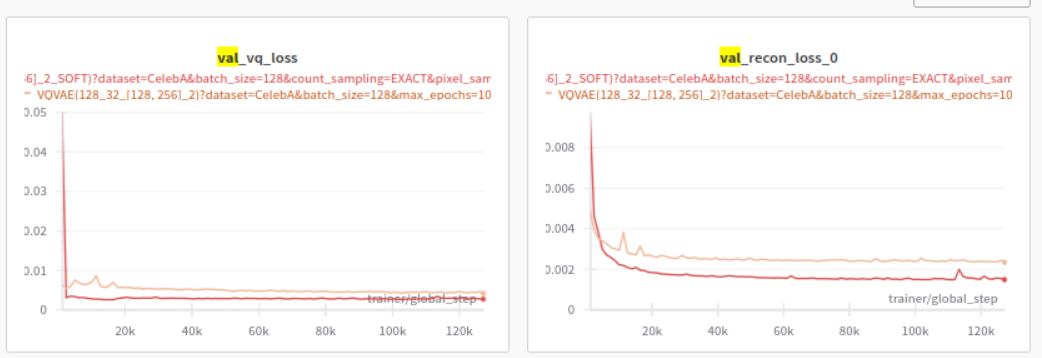
\includegraphics[width=0.8\textwidth]{figures/results/VQ+RECON.png}
    \caption[Validation loss comparison during training of a Gaussian VAE.]
    {
        Validation losses during training with and without \methodOne{1} applied on VQ-VAE.
        Left: VQ objective loss comparison. Right: Reconstruction loss comparison of the $Decoder_1$ - non-conditioned decoder.
    }
    \label{fig:results_method1_vq_vae}
\end{figure}

\section{Results of \methodTwo{2}}

In this section, I will present the results of \methodTwo{2} on both Gaussian VAEs and VQ-VAEs. The method was applied to the same datasets as the previous method. For this method, I ran the experiments with both Uniform and Gaussian sampling. The count sampling was done with Power law distribution with different exponent values.

\subsection{Results on Gaussian VAEs}

The results showed that \methodTwo{2} can be used for unifying two decoders into one. The experiments were conducted with both Uniform and Gaussian sampling. The results showed that for both methods this comes at a cost of slightly lower quality of the reconstruction when no conditioning information is given compared to a standard Gaussian VAE. However, the findings showed that this approach can substantially reduce the KL divergence loss of the latent space, which can be seen in figure \ref{fig:results_method2_gaussian_vae}.

Although, for both Uniform and Gaussian sampling findings showed that this method results in a slightly lower quality of the reconstruction compared to a standard Gaussian VAE. This approach reduced the KL divergence loss of the latent space for both of the sampling methods. For Uniform sampling, the results showed that the KL divergence loss of the latent space was reduced more compared to Gaussian sampling. One possible explanation for this could be that with Gaussian sampling, there is a higher probability of sampling the same pixel multiple times, which can be less informative for the decoder.

Experiments were also conducted with a range of different exponent values for the power-law distribution. The findings showed that the higher the exponent value the more the model was able to reduce the reconstruction loss of the scenario, where no conditioning information is given. However, the KL divergence loss of the latent space increased with higher exponent values.

\begin{figure}[H]
    \centering
    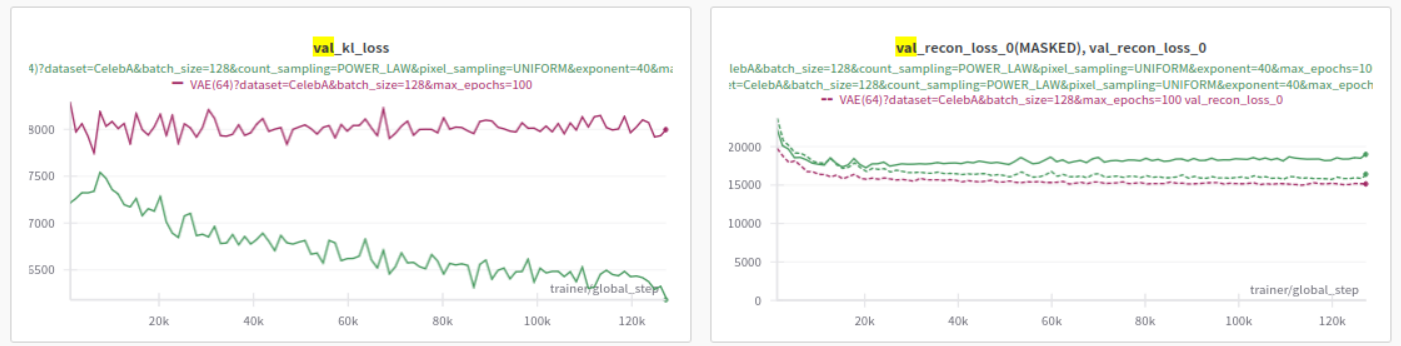
\includegraphics[width=0.8\textwidth]{figures/results/scvae1d/KL_and_recon.png}
    \caption[Validation loss during training with \methodTwo{2} applied on Gaussian VAE.]
    {
        Validation losses during training with and without \methodTwo{2} applied on Gaussian VAE.
        Left: KL loss comparison. Right: Reconstruction loss comparison of the $Decoder_1$ - non-conditioned decoder with a standard Gaussian VAE.
    }
    \label{fig:results_method2_gaussian_vae}
\end{figure}

\subsection{Results on VQ-VAEs}

The results showed that \methodTwo{2} worked very well with VQ-VAEs. The results showed it can be used to substantially reduce the VQ objective loss and at the same time to improve the quality of the reconstruction when no conditioning information is given. This showed to be the case for both Uniform and Gaussian sampling with a high enough exponent value for the power-law distribution.

The experiments were run with a range of different exponent values: 20, 30, 40, 50, 60. The results showed that the higher the exponent value the better the reconstruction in the scenario where no conditioning information is given, which is expected since the higher the exponent value the less number of pixels are given to the decoder as conditioning information on average.

When comparing Uniform and Gaussian sampling, the results showed that Gaussian sampling performed slightly better than Uniform sampling. This can be explained by the fact that the information around the center of the image is more important for the reconstruction, which is more likely to be sampled with Gaussian sampling.

\begin{figure}[H]
    \centering
    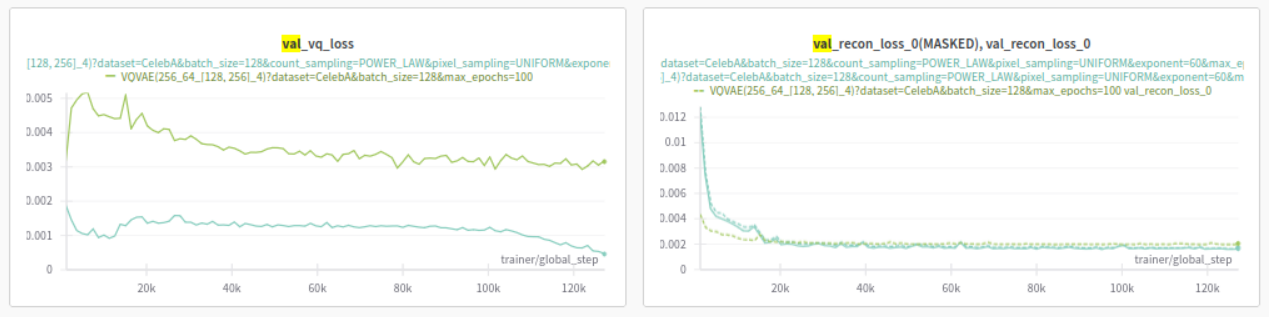
\includegraphics[width=0.8\textwidth]{figures/results/scvqvae1d/VQ_and_recon.png}
    \caption[Validation loss comparison during training of a VQ-VAE.]
    {
        Validation losses during training with and without \methodTwo{2} applied on VQ-VAE.
        Left: VQ objective loss comparison. Right: Reconstruction loss comparison of the $Decoder_1$ - non-conditioned decoder with a standard VQ-VAE.
    }
    \label{fig:results_method2_vq_vae}
\end{figure}

\section{Cross-validation results}

